\section{Results}
\label{sec:results}
The results follow the endpoints: first the primary contrast of the two fixed orders, then the per-class recall changes behind it, and finally the model checks. The balanced arm reaches 72.06 percent balanced accuracy (70.68 to 73.31). The reused arms reproduce the damages of the prevalence study: 0.57 points (0.30 to 0.84) at $\rho=10$, 2.91 points (2.48 to 3.34) at $\rho=100$, and 1.18 points (0.85 to 1.48) for the native allocation.

\subsection{Easy-tail and hard-tail orders}
\label{sec:contrast-results}
The easy-tail order costs 2.41 points (1.95 to 2.85) and the hard-tail order 1.59 points (1.22 to 1.95). Their difference is 0.82 points (0.24 to 1.39). The interval excludes zero and has the sign that headroom predicts, but the point estimate lies below the one-point threshold, and the interval contains values on both sides of it. Placing the classes with the most recall to lose at the smallest allocations thus costs slightly more than the reverse, by an amount the study does not resolve against the threshold.

The larger finding is that both fixed orders cost less than the random orders of the prevalence study. The easy-tail order lies 0.51 points (0.11 to 0.93) below the r100 damage, and the hard-tail order 1.33 points (0.87 to 1.78) below it, which is material. Across the 30 random orders of r100, the damage of a single draw ranges from 1.53 to 4.69 points (standard deviation 0.69), so both sorted orders fall at the low end of what random assignments produce (Figure~\ref{fig:spread}). Sorting the classes by difficulty, in either direction, is therefore not the worst assignment but among the mildest.

\begin{figure}[htbp]
\centering
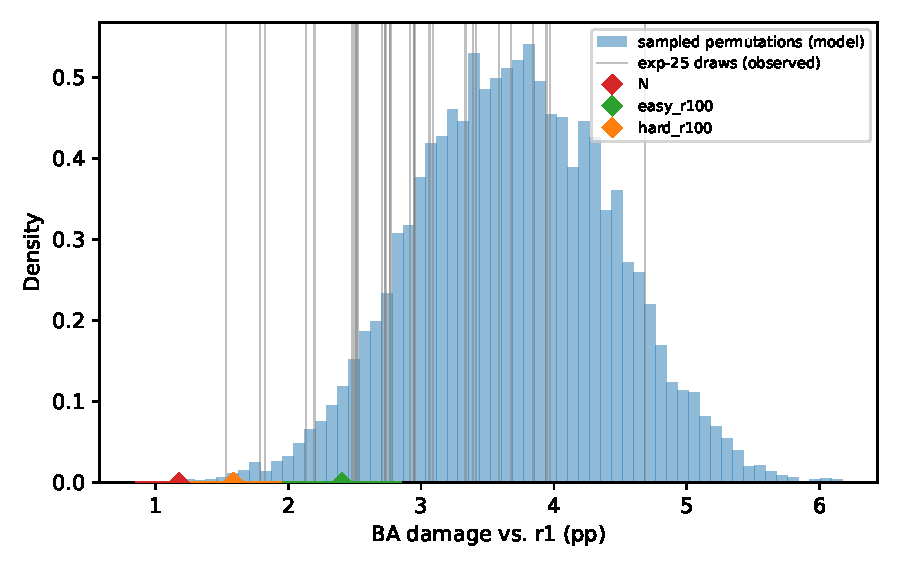
\includegraphics[width=0.75\textwidth]{assignment_spread_r100.pdf}
\caption{Both sorted orders cost less than a typical random order, and the model places the random-order damage too high. Histogram: damage predicted by the per-class allocation model for 10,000 random class orders at $\rho=100$. Grey lines: observed damage of each of the 30 random orders of the prevalence study. Diamonds with 95\% bootstrap intervals: observed damage of the easy-tail (green) and hard-tail (orange) orders at $\rho=100$, and of the native allocation (red, realized ratio 18.1, shown for reference). All damages are balanced-accuracy losses against the balanced arm, in points.}
\label{fig:spread}
\end{figure}

\subsection{Per-class recall under the two orders}
\label{sec:perclass-results}
Table~\ref{tab:perclass} lists each class's own recall change in both orders. Grouping the classes into thirds by balanced recall, the damage splits as follows. In the easy-tail order, the ten hardest classes, placed at ranks 0 to 9, gain 0.80 points of balanced accuracy (0.49 to 1.11), the middle ten at ranks 10 to 19 lose 1.49 points (1.25 to 1.72), and the ten easiest at ranks 20 to 29 lose 1.71 points (1.49 to 1.96). In the hard-tail order, the ten hardest classes at the tail lose 2.92 points (2.69 to 3.16), while the middle ten gain 0.54 points (0.37 to 0.72) and the ten easiest at the head gain 0.79 points (0.60 to 1.00).

\begin{table}[htbp]
\centering
\small
\setlength{\tabcolsep}{4pt}
\renewcommand{\arraystretch}{1.08}
\begin{tabular}{@{}lrlrrrrrr@{}}
\toprule
 & & & \multicolumn{3}{c}{Easy-tail order} & \multicolumn{3}{c}{Hard-tail order} \\
\cmidrule(lr){4-6}\cmidrule(lr){7-9}
Class & r1 recall & Partner & Rank (patches) & $\Delta$ & $\hat\Delta$ & Rank (patches) & $\Delta$ & $\hat\Delta$ \\
\midrule
ESCA & 28.2 & HNSC & 0 (2,843) & 18.2 & 25.0 & 29 (28) & $-$13.5 & $-$17.5 \\
CESC & 46.7 & LUSC & 1 (2,426) & 6.8 & 18.3 & 28 (33) & $-$18.9 & $-$17.7 \\
BLCA & 47.2 & LUSC & 2 (2,070) & 6.5 & 8.8 & 27 (39) & $-$15.3 & $-$20.9 \\
STAD & 47.2 & ESCA & 3 (1,766) & 1.9 & 12.0 & 26 (46) & $-$11.6 & $-$15.4 \\
COAD & 51.5 & READ & 4 (1,506) & 9.0 & 11.2 & 25 (54) & $-$11.4 & $-$20.6 \\
LUSC & 54.5 & HNSC & 5 (1,285) & 0.9 & 8.6 & 24 (63) & $-$9.7 & $-$23.4 \\
READ & 60.6 & COAD & 6 (1,097) & $-$13.4 & 6.8 & 23 (74) & 6.6 & $-$23.5 \\
SKCM & 62.6 & UVM & 7 (936) & 1.2 & 3.2 & 22 (86) & $-$10.2 & $-$13.0 \\
UCEC & 63.2 & STAD & 8 (798) & $-$4.3 & 1.4 & 21 (101) & $-$3.5 & $-$14.6 \\
LUAD & 65.3 & LUSC & 9 (681) & $-$3.0 & 0.4 & 20 (119) & $-$0.1 & $-$9.7 \\
\addlinespace
UCS & 68.4 & UCEC & 10 (581) & $-$0.5 & 0.7 & 19 (139) & $-$1.4 & $-$7.1 \\
HNSC & 69.0 & LUSC & 11 (496) & $-$11.9 & $-$2.7 & 18 (163) & 7.9 & $-$11.9 \\
BRCA & 70.4 & BLCA & 12 (423) & $-$8.2 & $-$3.2 & 17 (191) & 0.1 & $-$8.4 \\
PAAD & 70.8 & STAD & 13 (361) & $-$7.4 & $-$3.2 & 16 (224) & 4.6 & $-$6.7 \\
ACC & 72.9 & LIHC & 14 (308) & 0.7 & $-$3.0 & 15 (263) & $-$0.9 & $-$4.2 \\
MESO & 74.9 & BRCA & 15 (263) & $-$3.9 & $-$4.3 & 14 (308) & 1.9 & $-$3.5 \\
OV & 75.7 & UCEC & 16 (224) & $-$10.8 & $-$8.1 & 13 (361) & 3.3 & $-$5.1 \\
GBM & 77.0 & LGG & 17 (191) & $-$1.0 & $-$5.2 & 12 (423) & 0.6 & $-$1.3 \\
LGG & 78.8 & GBM & 18 (163) & 0.3 & $-$3.3 & 11 (496) & 1.1 & 0.3 \\
KIRP & 80.1 & KIRC & 19 (139) & $-$1.9 & $-$5.4 & 10 (581) & $-$0.8 & $-$0.2 \\
\addlinespace
SARC & 80.3 & UCS & 20 (119) & $-$9.5 & $-$10.6 & 9 (681) & 1.2 & $-$0.5 \\
UVM & 84.7 & SKCM & 21 (101) & $-$3.9 & $-$5.0 & 8 (798) & 5.9 & 1.8 \\
LIHC & 85.5 & ACC & 22 (86) & $-$5.2 & $-$6.9 & 7 (936) & 2.3 & 1.4 \\
KIRC & 86.9 & KIRP & 23 (74) & $-$1.9 & $-$3.3 & 6 (1,097) & 0.3 & 1.3 \\
TGCT & 88.2 & UCS & 24 (63) & $-$5.2 & $-$3.4 & 5 (1,285) & 4.2 & 3.0 \\
KICH & 93.1 & KIRC & 25 (54) & $-$4.4 & $-$5.4 & 4 (1,506) & 0.9 & 3.2 \\
THYM & 94.0 & CESC & 26 (46) & $-$7.3 & $-$5.8 & 3 (1,766) & 3.2 & 1.9 \\
PCPG & 94.3 & LGG & 27 (39) & $-$4.7 & $-$4.3 & 2 (2,070) & 2.1 & 1.8 \\
PRAD & 94.8 & BRCA & 28 (33) & $-$4.4 & $-$2.1 & 1 (2,426) & 2.0 & 1.2 \\
THCA & 95.1 & KIRP & 29 (28) & $-$4.9 & $-$3.9 & 0 (2,843) & 1.6 & 2.2 \\
\bottomrule
\end{tabular}
\caption{The model misses the recall changes of classes whose main confusion partner sits at a very different rank. For each class (TCGA project code), ordered by balanced-arm recall in percent: its main confusion partner, the class that receives the largest share of its off-diagonal confusion mass in the balanced arm; and, for each order, its rank with the patch count at that rank, its observed change of own patient-macro recall against the balanced arm ($\Delta$), and the change predicted by the per-class allocation model ($\hat\Delta$), both in points of recall and pooled over 30 fits. Rules separate the thirds of classes by balanced recall.}
\label{tab:perclass}
\end{table}

\noindent The middle third isolates the effect of the other classes. Its ten classes occupy ranks 10 to 19 in both orders, only mirrored, so as a group they receive the same ten allocations. Their summed own loss nevertheless differs by 2.03 points of balanced accuracy between the orders, with non-overlapping intervals, while the model predicts 1.25 points of loss in the easy-tail order and 1.60 in the hard-tail order. Which ranks the other classes hold therefore moves the middle third by more than the whole primary contrast.

The largest deviations concern pairs of classes that the balanced classifier confuses with each other. In the balanced arm, 36.1 percent of colon adenocarcinoma (COAD) test patches are predicted as rectum adenocarcinoma (READ), and 27.1 percent of READ patches as COAD; glioblastoma (GBM) and lower-grade glioma (LGG) exchange about 14.5 percent in each direction, and head and neck squamous cell carcinoma (HNSC) sends 12.2 percent to lung squamous cell carcinoma (LUSC). In the easy-tail order READ sits at rank 6 with 1,097 patches, above balance, but two ranks below COAD with 1,506 patches, and it loses 13.4 points of recall where the model predicts a gain of 6.8. In the hard-tail order READ sits at rank 23 with only 74 patches, but above COAD with 54, and it gains 6.6 points where the model predicts a loss of 23.5. HNSC shows the same pattern: it loses 11.9 points at rank 11 in the easy-tail order, below its partner LUSC at rank 5, and gains 7.9 points at rank 18 in the hard-tail order, above LUSC at rank 24. GBM and LGG, which sit at adjacent ranks in both orders, change by at most 1.1 points in either. A class's recall thus follows its allocation relative to its confusion partners more than its absolute allocation.

The easy classes of TCGA-UT do not collapse in the tail. In the easy-tail order, the ten easiest classes lose between 1.9 and 9.5 points of recall at ranks 20 to 29, with 28 to 119 patches, and thyroid carcinoma (THCA) at the tail keeps 90.2 percent. The hard classes lose more at the same ranks in the hard-tail order, between 3.5 and 18.9 points for eight of the ten; esophageal carcinoma (ESCA) at the tail keeps 14.8 of its 28.2 percent. The positive primary contrast therefore does not arise because easy classes lose everything in the tail, as on BRACS. It arises because, in the easy-tail order, the confusable middle classes lose recall to better-allocated partners, whereas in the hard-tail order the hard classes lose recall mostly among each other.

\subsection{Model checks}
\label{sec:model-results}
The per-class allocation model fits the stored fits it was built from reasonably well, with an $R^2$ of 0.73 for the per-fit, per-class recall changes of the four reused arms, but it does not generalize. Leave-one-draw-out, the predicted and observed r100 damages of the 30 random orders are uncorrelated (Spearman 0.04, Pearson $-0.06$), with a mean absolute error of 0.85 points against an observed standard deviation of 0.69. The model also places the r100 damage too high: 3.51 points on average in leave-one-draw-out prediction and 3.69 points over the 10,000 sampled orders, against the observed 2.91 points. The piecewise-linear form thus misses the curvature of the response between $\rho=10$ and $\rho=100$.

Out of sample, the model predicts the two fixed orders in the wrong direction. It predicts $-0.25$ points ($-0.93$ to 0.56) for the easy-tail order, observed 2.41, and 6.90 points (6.24 to 7.49) for the hard-tail order, observed 1.59. The errors follow from Table~\ref{tab:perclass}: the model attributes to the hard classes large gains at the head and large losses in the tail, fit from random orders in which a hard class's confusion partner usually holds a different rank, and these gains and losses shrink when the partners move with them. For the ten easiest classes, which have few confusion partners, the model's predictions are close in both orders: a summed own loss of 1.69 predicted against 1.71 observed in the easy-tail order, and a gain of 0.57 predicted against 0.79 observed in the hard-tail order.

For the same reason, the sampled-permutation spread of the model is not a reliable estimate of how much the assignment moves the damage. It predicts a 95 percent range of 2.26 to 5.11 points at $\rho=100$ and $-0.13$ to 1.39 points at $\rho=10$. The model's predicted tail own loss correlates negatively with balanced recall ($-0.78$ at both ratios; 95\% interval $-0.85$ to $-0.69$ at $\rho=100$) and positively with confusability (0.71 at $
ho=100$, 0.74 at $
ho=10$), the pattern the overlap mechanism predicts (Figure~\ref{fig:tailloss}). Because these values inherit the confusion-partner confound of the random orders, they describe what a class loses in the tail when its partners are elsewhere, not what it costs in general.

\begin{figure}[htbp]
\centering
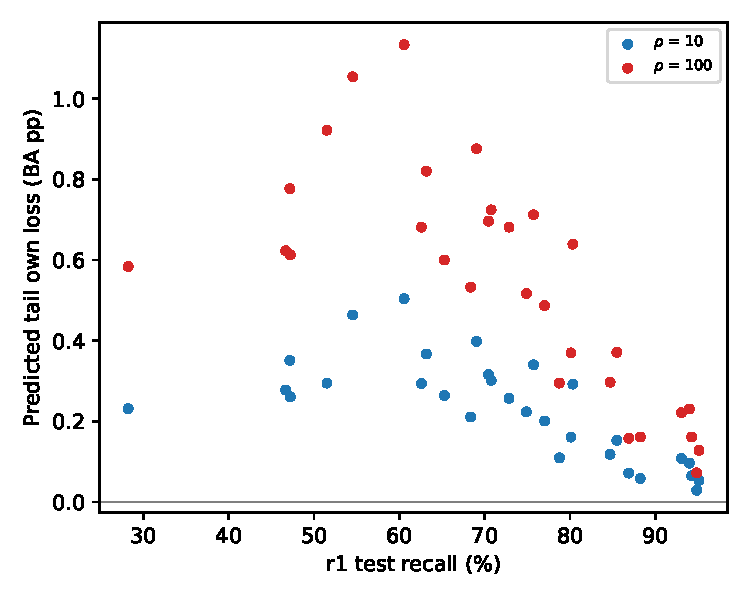
\includegraphics[width=0.55\textwidth]{tail_loss_vs_recall.pdf}
\caption{In random orders, hard classes lose more in the tail than easy classes. Predicted own loss of each class at rank 29 under the per-class allocation model, in points of balanced accuracy, against its balanced-arm recall, at $\rho=10$ (blue) and $\rho=100$ (red). The model is fit on the random orders of the prevalence study, in which a class's confusion partners usually sit at other ranks.}
\label{fig:tailloss}
\end{figure}

\noindent An exploratory extension, not specified before the Part B fits, adds to Equation~\eqref{eq:model} two piecewise slopes on the class's log-count relative to the confusion-weighted mean log-count of all other classes, with weights from the balanced-arm confusion matrix. It raises $R^2$ on the reused arms from 0.73 to 0.84 and shrinks the out-of-sample errors to 1.17 points for the easy-tail order (predicted 1.24) and 0.93 points for the hard-tail order (predicted 2.52), fit on point estimates without bootstrap intervals. It still ranks the hard-tail order above the easy-tail order and predicts the random draws poorly (leave-one-draw-out Spearman 0.15). Relative allocation to confusion partners thus explains a large part of the model's failure, but not enough to make the damage of an arbitrary assignment predictable.

\section{Discussion}
\label{sec:discussion}
On TCGA-UT, which classes sit in the tail changes the damage at $\rho=100$ by about one point, far less than on BRACS. Placing the easy classes in the tail costs 0.82 points more than placing the hard classes there, with the sign headroom predicts, but below the practical threshold. Both sorted orders cost less than a random order, by 0.51 and 1.33 points. The single observed random orders span 1.53 to 4.69 points, a wider range than the contrast, although this range also contains the variation of patients and test sets between draws.

The mechanism differs from the BRACS one. On BRACS, almost every class collapsed to near-zero recall in the tail, so a class cost what it had to lose \citep{queisler2026tailBracs}. On TCGA-UT, the easiest classes keep about 90 percent recall with 28 to 119 patches, and the hard classes, not the easy ones, lose the most own recall in the tail. What decides a class's recall is its allocation relative to the classes it is confused with: READ loses 13 points above balance when COAD has more patches and gains 7 points far below balance when COAD has fewer. This is consistent with the prior-versus-support study, in which the skewed class prior carried most of the TCGA-UT damage \citep{queisler2026causeTcga}: a shifted prior moves the decision boundary between two overlapping classes toward the rarer one, and it matters little when neither class has a close neighbour. A random order often separates confusion partners, placing one at the head and the other in the tail; a sorted order keeps partners of similar difficulty close in rank, so their priors shift together and the boundary between them moves less. This explains why both sorted orders cost less than random ones and why the hard-tail order, which keeps the confusable squamous and gastrointestinal classes together at the tail, costs least.

For the question of the worst tail assignment, the results point away from difficulty or headroom alone. On TCGA-UT, the damage of an assignment depends on pairs: it is largest when confusion partners are separated in rank, with the member that has more recall to lose placed lower. An assignment built from the balanced-arm confusion matrix, giving one member of each strongly confused pair the head and the other the tail, is the natural candidate for the worst case. This report does not fit it; the exploratory partner model gives only a rough indication of its size.

The per-class allocation model fails as a substitute for fitting. It describes the random orders it was fit on, but its predictions do not track the damage of held-out random orders and invert the ordering of the two fixed orders. The failure has a clear cause, the missing dependence on other classes' allocations, and adding a confusion-weighted relative allocation reduces but does not remove it. For the design of imbalance studies, this supports averaging the damage over random class orders, as the prevalence curve does: a single fixed order can land more than a point from the average, and no simple per-class model corrects for it.

\section{Limitations}
\label{sec:limitations}
Part B tests two fixed orders at one ratio, and each order is the same in all 30 draws; its damage therefore reflects one assignment, and the contrast between the two orders cannot be separated from the specific class pairings that each sorted order produces. The sorted orders move every class at once, so the contrast is not a test of a single tail class. The per-class recall changes in Table~\ref{tab:perclass} are pooled point estimates; the interpretation of individual classes rests on changes of about 10 points or more, well above their interval half-widths of about 1 to 6 points. The range of observed single-draw damages contains both assignment and draw variation and overstates the effect of the assignment alone.

The confusion-partner reading was formed after the Part B fits, and the partner model that supports it was specified afterwards and fit without bootstrap intervals, so it is exploratory. Confusion partners are defined from pooled patch-level confusion counts in the balanced arm, which weight classes with many test patches more heavily and do not capture morphological similarity as a pathologist would rate it. All results are conditional on twenty patients per class, frozen Virchow2 features, multinomial logistic regression, and the three overlapping splits of TCGA-UT.
